\documentclass{beamer}
\usepackage{mathrsfs,xcolor,setspace,comment,centernot,listings,framed,subfig,ragged2e}
\usepackage[utf8]{inputenc}
\usepackage[T1]{fontenc}

\DeclareMathOperator{\Cov}{Cov}
\DeclareMathOperator{\Var}{Var}
\DeclareMathOperator{\E}{\mathbb{E}}
\DeclareMathOperator{\Proba}{\mathbb{P}}

\newcommand{\Covb}[2]{\ensuremath{\Cov\!\left[#1,#2\right]}}
\newcommand{\Eb}[1]{\ensuremath{\E\!\left[#1\right]}}
\newcommand{\Pb}[1]{\ensuremath{\Proba\!\left[#1\right]}}
\newcommand{\Varb}[1]{\ensuremath{\Var\!\left[#1\right]}}

% norm
\newcommand{\norm}[1]{\| #1 \|}

\newcommand{\indep}{\rotatebox[origin=c]{90}{$\models$}}



% config du theme metropolis
\usetheme[progressbar=frametitle,block=fill, titleformat=smallcaps,sectionpage=progressbar,]{metropolis}


\title{A new geospatial vector data matching algorithm optimised for building change detection}
\subtitle{}

\date{11/03/2025\\
\textit{Journée de la Recherche UGE-IGN-ENSG 2025}\\
Session: \textit{Détection de Changement}}

\author{Juste Raimbault\textsuperscript{1,2,3,4}, Paul Guardiola\textsuperscript{1}, Julien Perret\textsuperscript{1,5} and  Ana-Maria Olteanu-Raimond\textsuperscript{1}}
\institute{\textsuperscript{1}LaSTIG, IGN-ENSG-UGE\\
\textsuperscript{2}CASA, UCL\\
\textsuperscript{3}UPS CNRS 3611 ISC-PIF\\
\textsuperscript{4}UMR CNRS 8504 Géographie-cités\\
\textsuperscript{5}LaDéHiS, EHESS
}



%definition de la couleur du texte dans la balise \alert{}
\definecolor{vertIGN}{HTML}{96C31E} % vert IGN %vrai valeur #97BE0D
\setbeamercolor{alerted text}{fg=vertIGN}

\definecolor{grisIGN}{HTML}{22292F} % Gris IGN tiré vers le noir 
\setbeamercolor{background canvas}{bg=grisIGN}


% code pour placer le log ENSG dans le bandeau de titre 
\makeatletter
\setbeamertemplate{frametitle}{%
  \nointerlineskip%
  \begin{beamercolorbox}[%
      wd=\paperwidth,%
      sep=0pt,%
      leftskip=\metropolis@frametitle@padding,%
      rightskip=\metropolis@frametitle@padding,%
    ]{frametitle}%
  \metropolis@frametitlestrut@start%
  \insertframetitle%
  \nolinebreak%
  \metropolis@frametitlestrut@end%
  \hfill
  \raisebox{-0.6ex}{
\includegraphics[height=4ex,keepaspectratio]{figures/logoENSG_small.jpg}}
  \end{beamercolorbox}%
}


\newcommand{\noun}[1]{\textsc{#1}}
\newcommand{\jitem}[1]{\item \begin{justify} #1 \end{justify} \vfill{}}
\newcommand{\sframe}[2]{\frame{\frametitle{#1} #2}}

\newenvironment{centercolumns}{\begin{columns}[c]}{\end{columns}}
%\newenvironment{jitem}{\begin{justify}\begin{itemize}}{\end{itemize}\end{justify}}



\usepackage{pifont}
\newcommand{\cmark}{\ding{51}}
\newcommand{\xmark}{\ding{55}}


\usepackage{multirow}

\makeatother




% logo ENSG première page 
\titlegraphic{\vspace{4cm}\flushright
\includegraphics[width=2cm,height=2cm]{figures/logoENSG_big.png}} 





\begin{document}
\metroset{background=dark} % change background theme according to manual
\maketitle	



% Change detection using vector data is challenging when data specification and quality are not stable in time, as for example with buildings in BDTOPO with a time interval including 2015. Therefore, vector data matching algorithms can be used to remove such noise and accurately detect newly constructed entities. Such algorithms have however various case-dependant performances, and need to be parametrised. We describe a new algorithm with combines Geometric Matching of Areas and Multi-Criteria Matching algorithms, using the appropriate option on the type of potential links for which it performs best. We integrate the algorithm into the OpenMOLE platform, to optimise its performance for building change detection on ground-truth datasets of four case studies cities (Strasbourg, Toulouse, Dortmund, Frankfurt) between 2011 and 2021.

\sframe{Context: the SUBDENSE project}{

\medskip

\begin{columns}
	\begin{column}{0.6\textwidth}
		The SubDense European project studies the dynamics of suburban densification by:
 
	\end{column}
	\begin{column}{0.4\textwidth}
		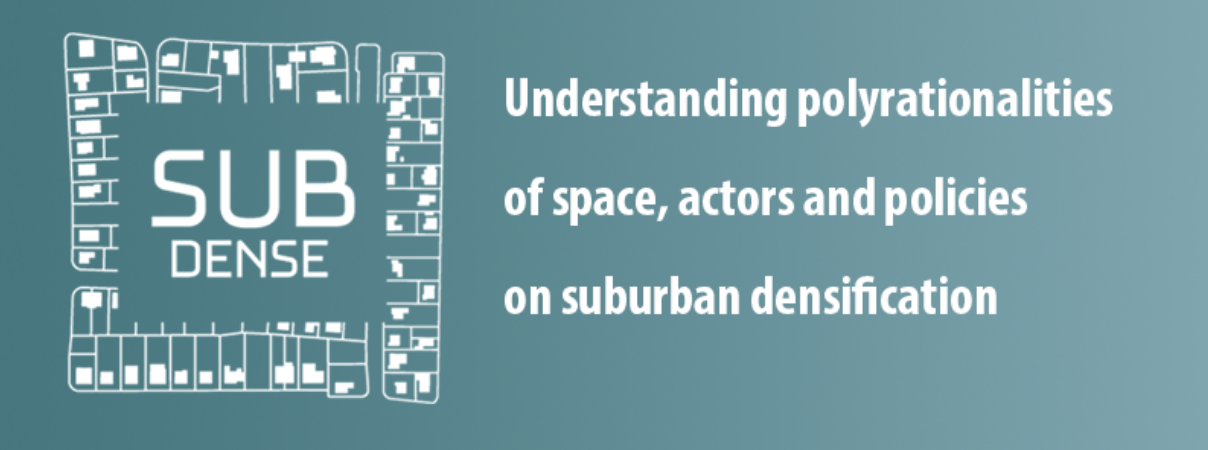
\includegraphics[height=0.2\textheight]{figures/subdense.png}
	\end{column}
\end{columns}


\begin{itemize} 
	\item exploring how diverse strategies of land policy interact with landowners’ and local stakeholders’ interest and agency to shape suburban densification and their impact on suburbia across different planning systems (France, Germany, UK);
	\item combining quantitative approaches (geodata analysis and geosimulation) with qualitative approaches (social and policy science and planning).
\end{itemize}

\bigskip

\centering


\includegraphics[height=0.1\textheight]{figures/logos.png}\hspace{-0.1cm}

\includegraphics[height=0.1\textheight]{figures/tud.png}


}

\sframe{A collaborative dashboard for mediation}{

\begin{columns}

\begin{column}{0.6\linewidth}

\bigskip

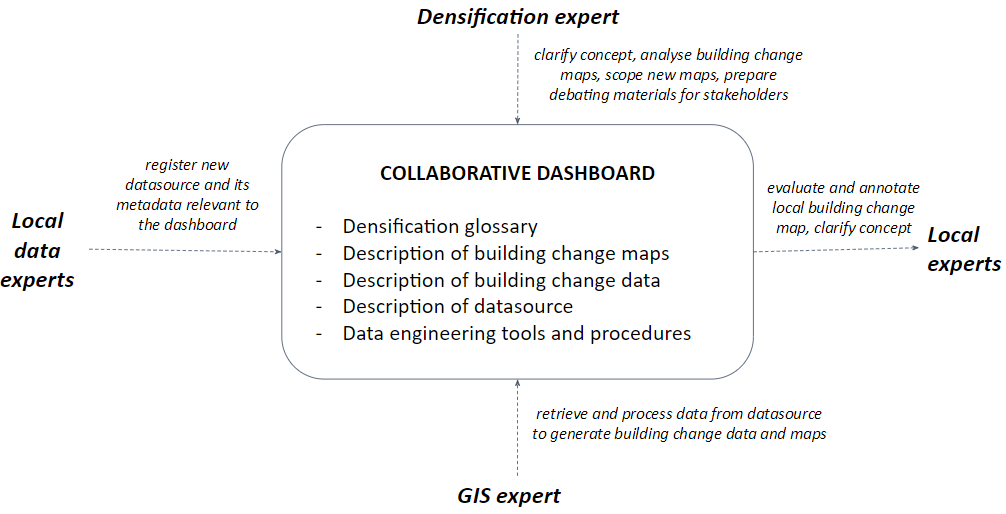
\includegraphics[width=\linewidth]{figures/dashboard_concept.png}\smallskip

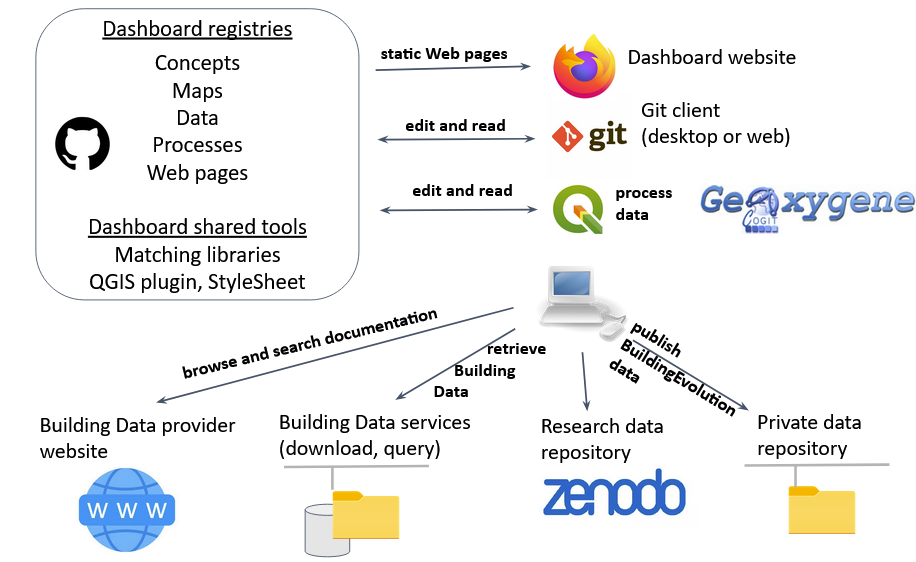
\includegraphics[width=\linewidth]{figures/dashboard.png}

\end{column}
\begin{column}{0.4\linewidth}
	
	\footnotesize	
	
	$\rightarrow$ git-based dashboard to share knowledge and resources between different types of experts	\cite{bucher2024conceptualising}
	
	\bigskip
	
	$\rightarrow$ reproducible tools and methods, including \textbf{building change detection scripts} 	
	
\end{column}

\end{columns}

}


\sframe{Difficulties with vector data for building change}{

\begin{center}
	
	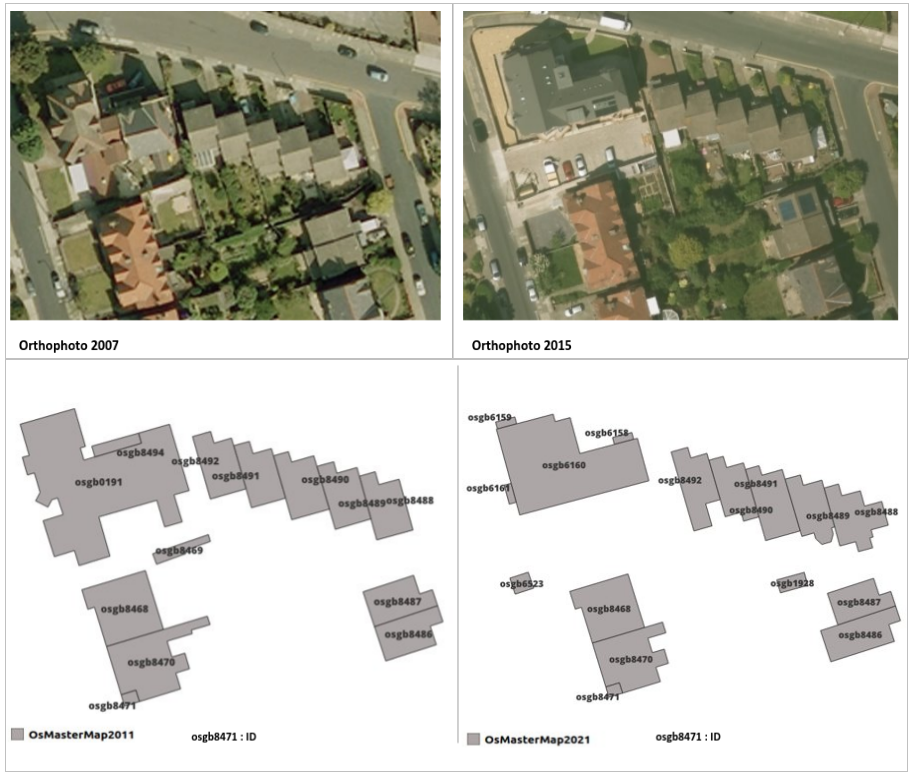
\includegraphics[width=0.75\linewidth]{figures/buildingchange_1.png}	
	
\end{center}

\footnotesize

\textit{Example in the UK where changes in OSMasterMap building data includes both real changes and data changes.} Source: \cite{bucher2025building}

}


\sframe{Difficulties with vector data for building change}{

\begin{center}
	
	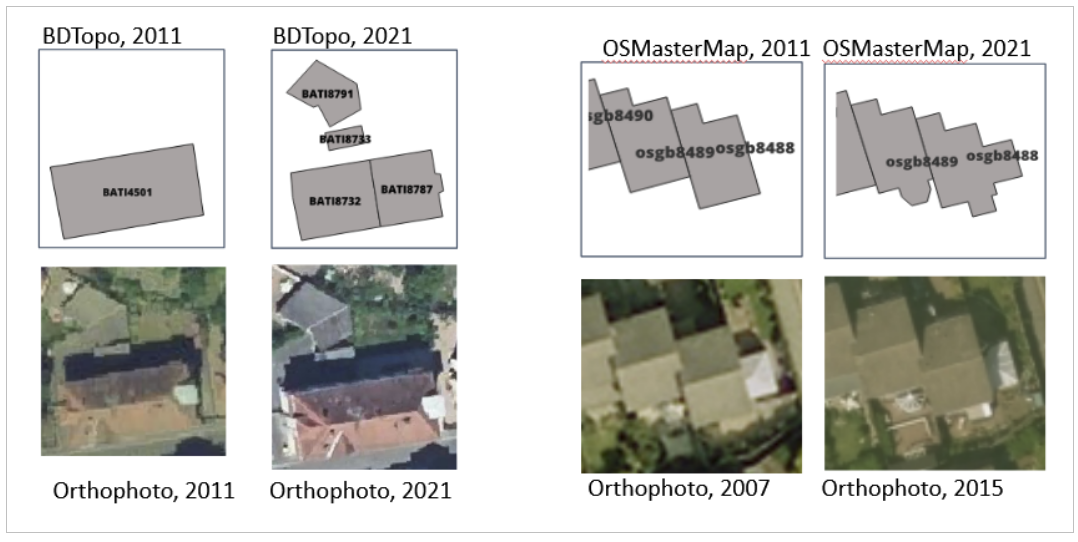
\includegraphics[width=\linewidth]{figures/buildingchange_2.png}	
	
\end{center}

\footnotesize

\textit{Example of data specification changes only, for France (BDTopo) and the UK (OSMasterMap).} Source: \cite{bucher2025building}

}

\sframe{Research objective}{

% a bit of lit here on matching for change detection

$\rightarrow$ Geospatial vector data matching algorithms as a method for change detection \cite{xavier2016survey}, applied to linear data \cite{costes2015aggregated} and polygonal data \cite{gregory2007historical}.

\medskip

$\rightarrow$ Several algorithms which have been developed and tested for different application (change detection, data quality) and different contexts, with meta-parameters for each.


\bigskip

\textbf{Research objective: }

\textit{Which algorithm and parametrisation are optimal to detect true building changes, across the three case study countries and the various urban contexts within the study areas?}


}

\sframe{Geometric Matching of Areas (GMoA) algorithm}{

\begin{columns}
  \begin{column}{0.4\textwidth}
  		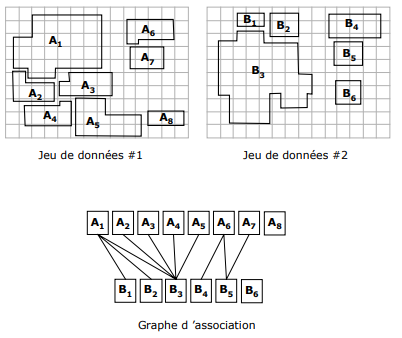
\includegraphics[width=\linewidth]{figures/GMoA_1.png}
	\smallskip
	  	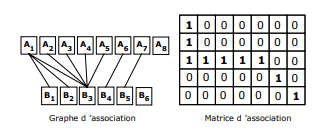
\includegraphics[width=\linewidth]{figures/GMoA_2.png}	
  		
  \end{column}
   \begin{column}{0.6\textwidth}
   
	\footnotesize   
   
  	 Algorithm to produce m-n links based only on geometries \cite{harvey1998geometric} \cite{belhadjali:tel-03244834}:
  	 
	\begin{enumerate}
		\item Construct all possible association links as surfaces with a non-empty intersection (top left Fig.)
		\item Filter links with an intersection surface below a threshold parameter
		\item Filter links with an intersection surface too small relatively to matched surfaces (rate parameter)
		\item Construct all m-n links as connected clusters in the remaining bipartite graph (bottom left Fig.)
	\end{enumerate}	  	 
  	 
  \end{column}
\end{columns}

\bigskip

\footnotesize

$\rightarrow$ implemented in the \texttt{geoxygene} java library \cite{bucher2012geoxygene} by \cite{mustiere2002description}



}

\sframe{Application of the GMoA to change detection}{

% -> code python shared through the dashboard

\begin{center}
  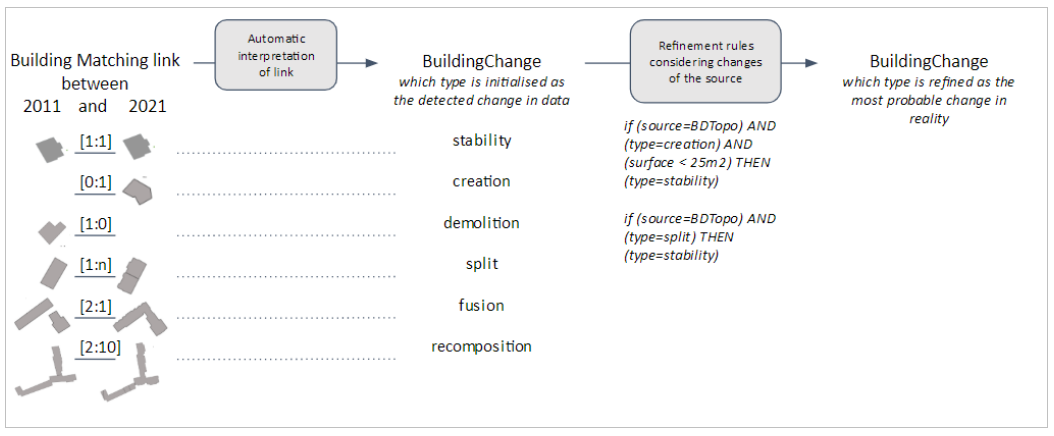
\includegraphics[width=\linewidth]{figures/change.png}
\end{center}

\bigskip

Automatic interpretation of matching links into building change, with specific adjustements for BDTopo \cite{bucher2025building}, by a \texttt{python} script available at \url{https://github.com/subdense/matching}


}


\sframe{Example}{

% Strasbourg?


\begin{center}
  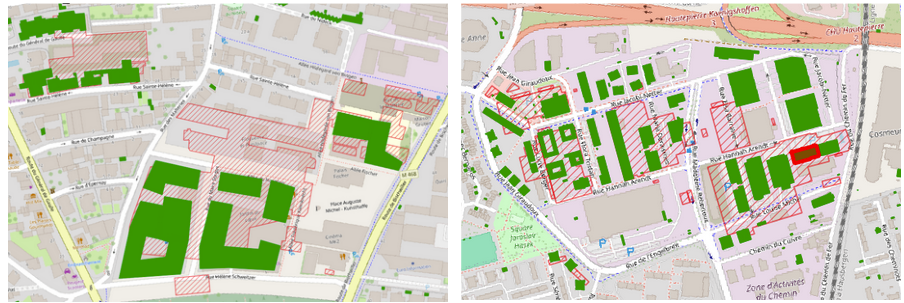
\includegraphics[width=\linewidth]{figures/buildingchange_gmoa.png}
\end{center}

\bigskip

Building evolution for two examples in the urban area of Strasbourg \cite{bucher2025building} 

}


\sframe{Multi-criteria matching algorithm (MCA)}{



\begin{center}
  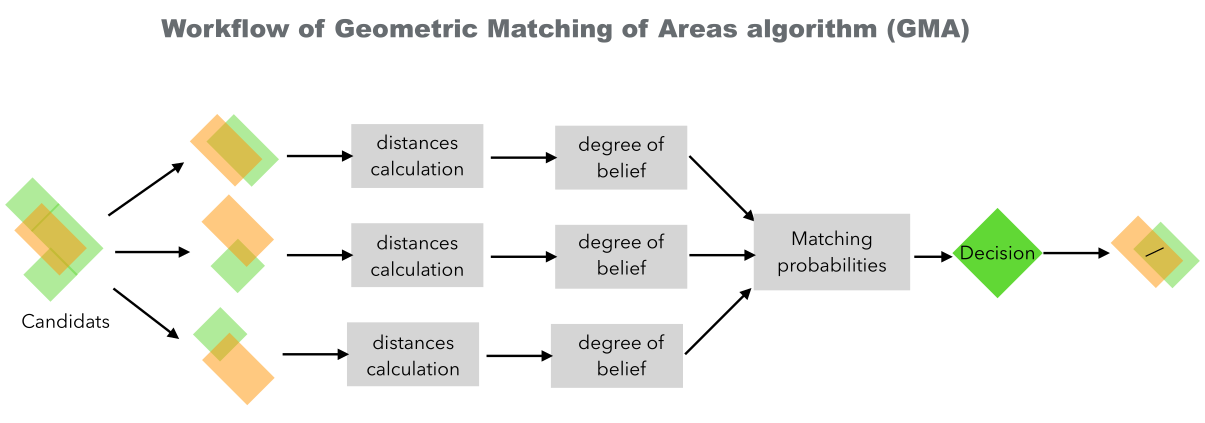
\includegraphics[width=\linewidth]{figures/mca.png}
\end{center}

\bigskip

Implementation of the Multi-criteria matching algorithm \cite{olteanu2015knowledge} in python by \cite{guardiola2024benchmarking}, with euclidian, surface, radial and Hausdorff distances, and run twice to obtain m-n links.

}


\sframe{Benchmarking of algorithms}{

% paper frccs 2024 -> optimal params for a compromise perf/time

\begin{center}
  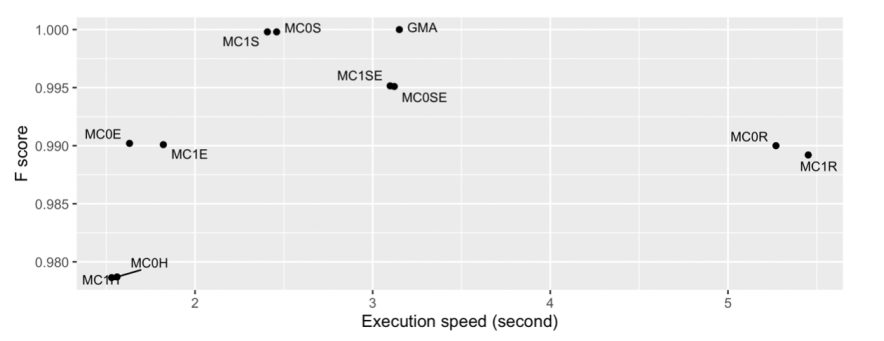
\includegraphics[width=\linewidth]{figures/benchmark.png}
\end{center}

\bigskip

\footnotesize

Bi-objective benchmark optimising for performance (F-score on a $\simeq$ 2k buildings ground truth dataset) and runtime, for different parametrisations of the two algorithms, by \cite{guardiola2024benchmarking}

$\rightarrow$ various algorithm performances

% We find an under-detection for the GMA and an over-detection for MCA
% GMA is a well method for n-m links rather than MCA is better for 1-1 links

$\rightarrow$ under-detection of change by GMoA and over-detection by MCA

$\rightarrow$ GMA better for m-n links, MCA better for 1-1 links


}


\sframe{A new algorithm using multi-modeling}{

% cite CCS2024

\begin{center}
  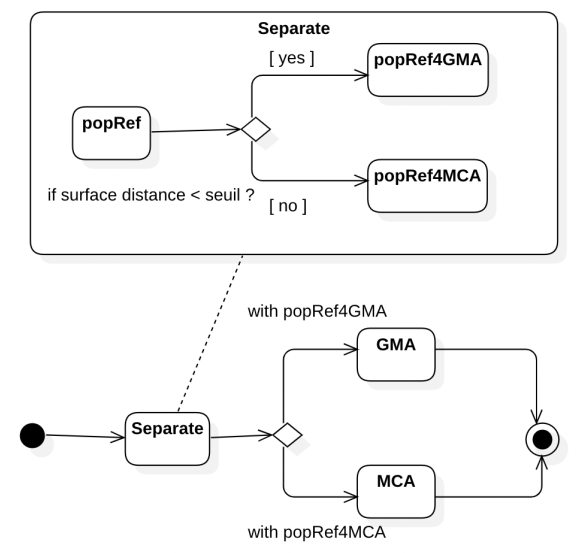
\includegraphics[width=0.6\linewidth]{figures/algo.png}
\end{center}

\bigskip

\footnotesize


Proposition of a new algorithm combining GMoA and MCA, with the choice made through thresholding surface distance \cite{guardiola2024optimising}

}


\sframe{Example}{

% Rennes


\begin{center}
  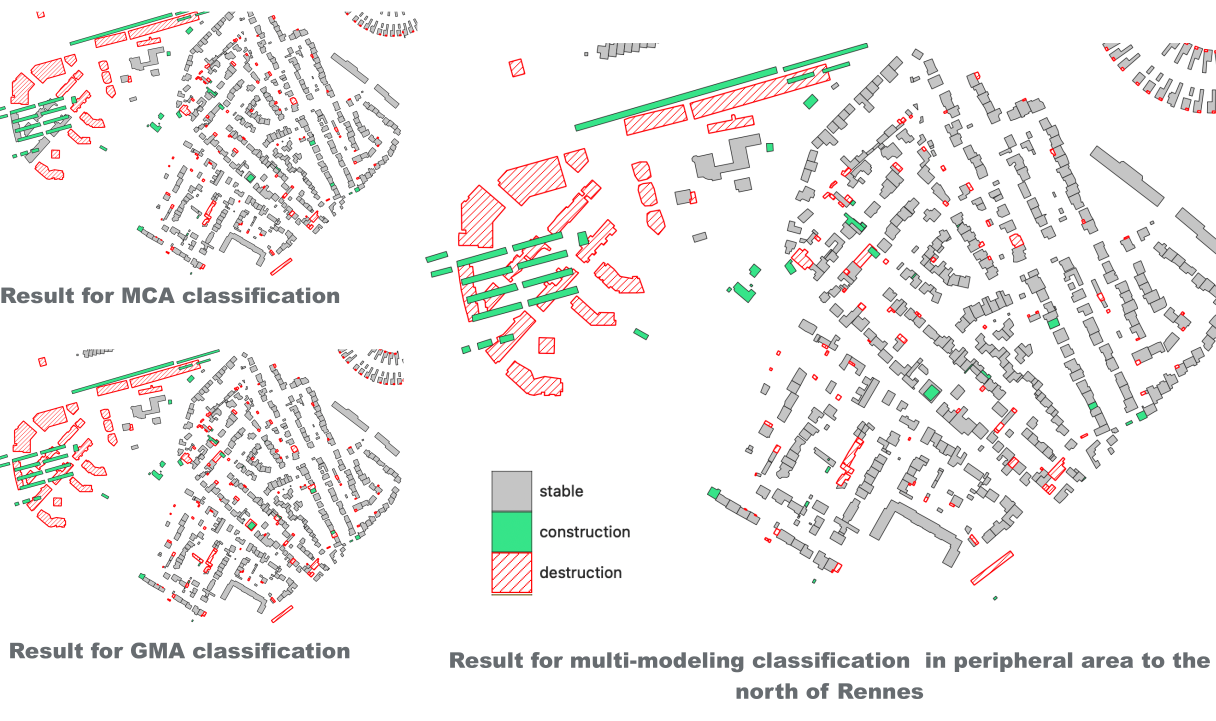
\includegraphics[width=\linewidth]{figures/result_algo.png}
\end{center}

\bigskip

%\footnotesize


Results obtained on an example in the suburbs of Rennes \cite{guardiola2024optimising}

}



\sframe{Validating the algorithm with synthetic data}{

% and optimising


\begin{center}
  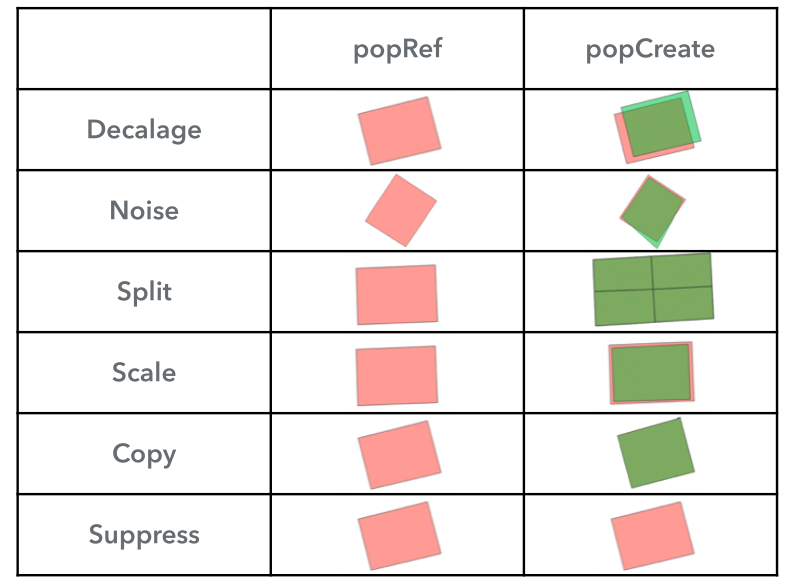
\includegraphics[width=0.63\linewidth]{figures/synthdata_1.png}
  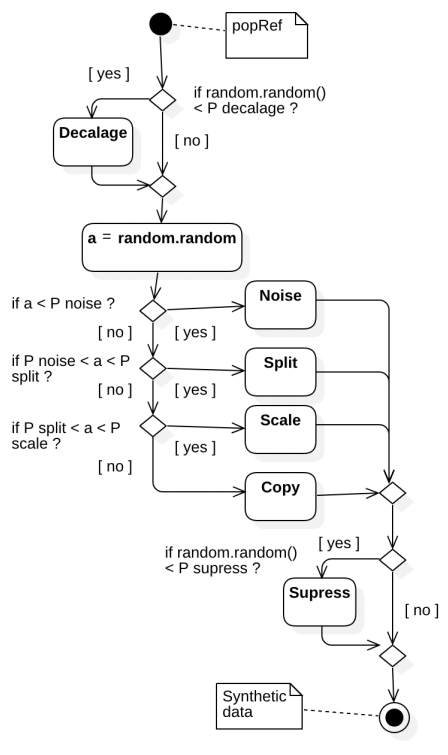
\includegraphics[width=0.27\linewidth]{figures/synthdata_2.png}
\end{center}

\bigskip

\footnotesize

Synthetic data generator introduced by \cite{guardiola2024optimising} to generate datasets on which to validate and optimise the algorithm

}


\sframe{First results on synthetic data}{

% integrated into OpenMOLE


\begin{center}
  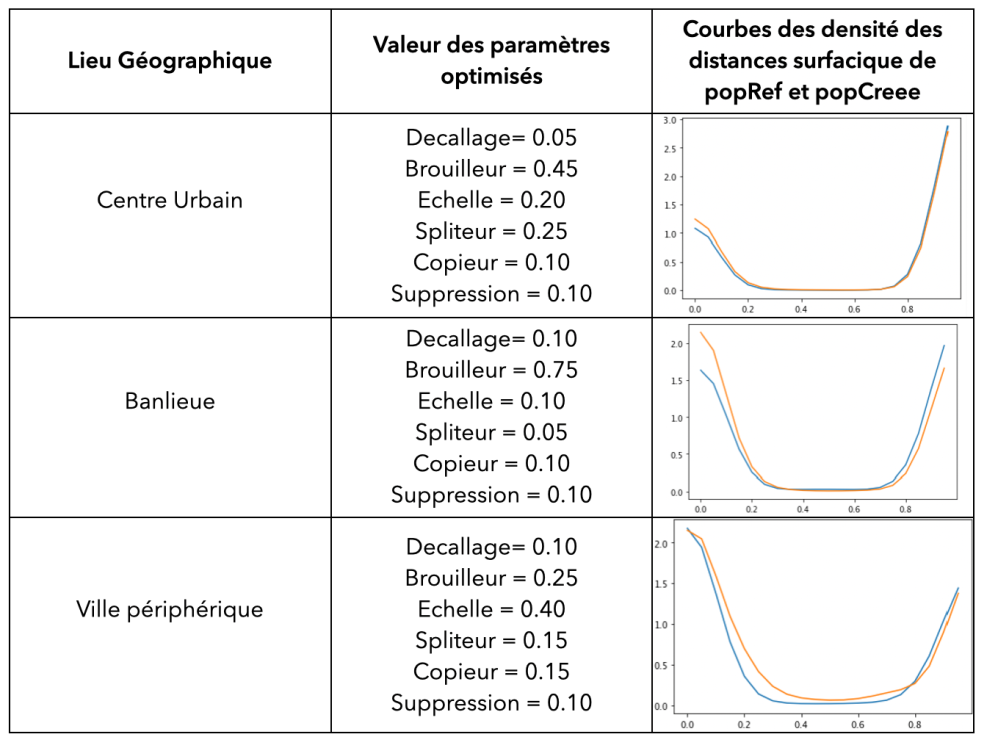
\includegraphics[width=0.75\linewidth]{figures/synthdata_calib.png}
\end{center}

\bigskip

\footnotesize

Integration into the OpenMOLE software and calibration of the generator for different urban typologies (single fitness: distance between surface distance densities) \cite{guardiola2024optimising}

}


\sframe{Validating the algorithm with ground truth data}{

% and optimising

% illustration annotator

% WIP optim with OpenMOLE

\begin{center}
  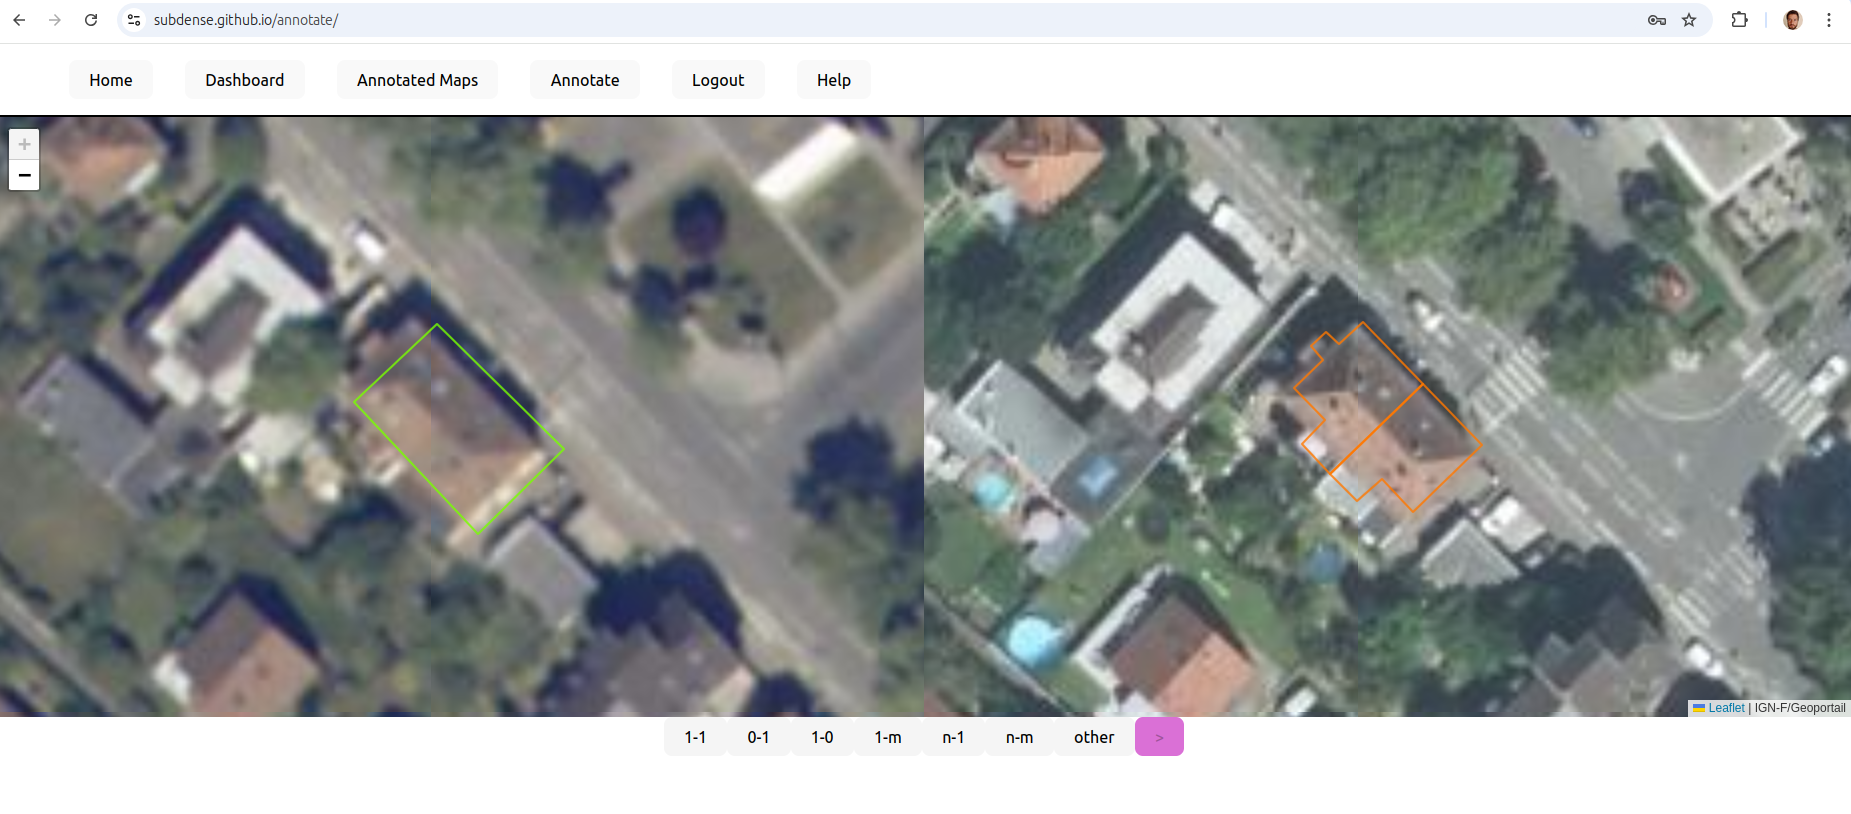
\includegraphics[width=\linewidth]{figures/annotator.png}
\end{center}

\smallskip

\footnotesize

Online standalone javascript app (deployed automatically via github pages) to annotate potential matching links (what link should be obtained; which real-world change), developped by Julien Perret (\url{https://github.com/subdense/annotate})

$\rightarrow$ work in progress: large annotation campaign for the 6 case study cities in the 3 countries


}


\sframe{Work in progress and perspectives}{

% pymatch lib
% ground truth datasets to be published
% optimise combined algo - benchmark systematically with others

\footnotesize

\textbf{Contributions: }

\begin{itemize}
	\item a benchmark of algorithms \cite{guardiola2024benchmarking}
	\item a new algorithm combining GMoA and MCA \cite{guardiola2024optimising}
	\item open source python library \url{https://github.com/umrlastig/pymatch}
	\item web app to annotate links \url{https://github.com/subdense/annotate}
\end{itemize}

\medskip

\textbf{Work in progress: } % aka necessary for solid paper

\begin{itemize}
	\item annotation campaign to produce a large scale ground-truth dataset
	\item optimisation using the ground truth in OpenMOLE
	\item systematic exploration and validation using the synthetic data generator
	\item include other matching algorithms in the benchmark % at least one well established in the literature
\end{itemize}

\medskip

\textbf{Perspectives: }

\begin{itemize}
	\item extension to line and points matching algorithms
	\item use for data quality issues
\end{itemize}



}







%%%%%%%%%%%%%%%%%%%%%
\begin{frame}[allowframebreaks]
\frametitle{References}
\bibliographystyle{apalike}
\bibliography{biblio}
\end{frame}
%%%%%%%%%%%%%%%%%%%%%%%%%%%%





\end{document}

